%Linea Para poder completar automaticamente las citas con el Sublime
%No hace el documento, se puede borrar esta linea si no se usa el Sublime
%------------------------------------------------------------------------------
 \newcommand{\NoBiblioMeso}[1]{
 \ifthenelse{\equal{#1}{verdadero}}{}{\bibliography{Referencias/base_bibliografica}}
 \NoBiblioMeso{verdadero}}
 %-----------------------------------------------------------------------------

%Formato (Nombre de capitulo largo o corto), nombre del capitulo, resumen y estilo de la
%Portada del Capitulo
%------------------------------------------------------------------------------
 
 %Formato en si, titulo en dos renglones
 \FormatoCapituloDosLineas
 
 %Nombre y etiquete para referir
 \chapter{Películas delgadas mesoporosas de óxido de silicio\index{silicio!oxido de}}
 \label{chap:Mesoporosos}

 %Para que no salga el numero de pagina en la portada del capitulo
 \thispagestyle{empty}
	
 %Resumen del Capitulo en Italica
 \noindent\textit{En capitulo explica como se sintetizaron y depositaron las películas mesoporosas sobre diferentes sustratos. El objetivo fue probar la capacidad de adherencia, homogeneidad y espesor a la hora de depositar películas de óxido de silicio\index{silicio!oxido de}\index{silicio} mesoporoso en una variedad de sustratos. Establecer y estudiar las técnicas de caracterización para evaluar y analizar la porosidad, accesibilidad, conectividad\index{conectividad} con el objetivo último de evaluar la factibilidad de utilizarlos como sensores\index{sensor} electroquímico\index{electroquimico}s\index{electroquimico}.}
 
 
 %Indice de capitulo alineada al borde inferior de la pagina, nueva pagina
 \vfill
 \minitoc
 \newpage
 %-------------------------------------------------------------------------------

\section{Introducción}

	Existen una gran variedad precursor\index{precursor}es para estructurar el esqueleto de películas mesoporosas de SiO$_2$, de Ti\index{titanio}O$_2$, Zr\index{zirconio}O$_4$, por enumerar los  óxidos más utilizados. También existe una gran variedad de agentes moldeante para establecer el tamaño y características de los poros (F127, P123, Brij 58, CTAB, etc). En este trabajo se trabajó exclusivamente con óxido de silicio\index{silicio!oxido de}\index{silicio} para generar la estructura inorgánica y con Pluronic F127\index{Pluronic F127} y bromuro de hexadeciltrimetilamonio\index{bromuro de hexadeciltrimetilamonio} (CTAB) para modelar el entramado poroso. Esta elección no fue arbitraria, sino que se hizo en base a premisas bien fundamentadas:
		\begin{enumerate}

		\item El SiO$_2$ es procesable por técnicas sol-gel\index{sol-gel} a través de diferentes precursor\index{precursor}es, es económico y fundamentalmente es el óxido mas utilizado en microelectrónica\index{microelectrónica}, aspecto fundamental en este trabajo para compatibilizar los procesos \textit{top-down}\index{top-down@\textit{top-down}} y \textit{bottom-up}\index{bottom-up@\textit{bottom-up}}.

		\item Ti\index{titanio}ene una química rica, bien conocida, forma enlaces covalentes y es fácilmente funcionalizable post-síntesis. Esta característica resultará fundamental para la selectividad de los sensores.

		\item No presenta absorción en el UV/Vis\index{UV}, esta característica es fundamental para poder hacer polimerizaciones dentro de los nanoporos sin tener interferencias por absorción de luz.

		\item Como agente moldeante\index{agente moldeante} se uso F127 y CTAB para tener películas con tamaño de poros bien variados, con diámetro aproximado de \SI{10}{\nm} para el F127 y de \SI{2}{\nm} para el CTAB.

		\end{enumerate}
	
	Finalmente, elegidos los componentes esenciales que darán estructura a la película activa, se hizo foco en variar los sustratos. Ya que, al ser el objetivo final de la tesis sentar las bases para la fabricación de sensores\index{sensor} multiselectivos, se debían explorar las distintos soportes para las películas mesoporosas, de forma de poder abarcar un rango amplio de materiales para distintos usos.

	Se depositaron los soles\index{sol} sobre silicio\index{silicio} monocristalino, sobre vidrio\index{vidrio} y sobre películas delgadas de Au. En esta primera etapa el objetivo era estudiar el comportamiento de las películas frente a diferentes sustratos. Para poder comparar los resultados con la bibliografía\cite{Soler-Illia2006,Brinker1990} se decidió depositar las películas por la ruta clásica de calcinación\index{calcinación} explicada en la pág. \pageref{sec:cond_y_extr}. Impuestas estas condiciones de temperatura, se eligieron sustratos térmicamente estables:\marginpar{Faltan algunas referencias en este apartado}
		\begin{itemize}

			\item \textit{Portaobjetos de Vidrio}. Se utilizó para todo tipo de experimentos exploratorios, por ejemplo para pruebas de deposito, cortes o diseños, ya que es el mas económico que disponemos, de superficie\index{superficie} plana y con la misma composición que el sol, lo cual minimiza el estrés térmico sustrato-película.

			\item \textit{Silicio monocristalino, orientación cristalina [100]}. Las películas depositadas sobre silicio\index{silicio} se utilizaron para obtener gráficos de espectroscopía de absorbancia IR, para hacer elipsoporisimetrías e imágenesSEM\index{SEM} principalmente, también para hacer una primera inspección visual de la calidad de las películas, ya que es más fácil de visualizar la misma que sobre otras superficie\index{superficie} como el Au\index{oro} o el vidrio. 

			\item \textit{Películas delgadas de Au}. Estos sustratos fueron destinado para las pruebas electroquímica\index{electroquimico}s\index{electroquimico}, evaluar fenómenos de transporte, accesibilidad\index{accesibilidad} y propiedades de permeoselectividad. También se utilizó para imagenes deSEM\index{SEM}.

			\end{itemize}
	
	En los siguientes capítulos, veremos que, se extiende el uso de los sustratos considerablemente, abarcando virtualmente a cualquier superficie\index{superficie} de baja rugosidad\index{rugosidad} cuyo material sea estable por encima de los \SI{130}{\celsius}, incluyendo materiales poliméricos flexibles.
		
	%Siempre con la idea de desarrollar un multisensor electroquímico\index{electroquimico}s\index{electroquimico} selectivo, especifico, integrado y escalable decidimos, para logra este fin, explorar las propiedades de las películas delgadas de óxidos mesoporosos descritas con anterioridad. Nos dedicamos, como primera aproximación, a depositar estas películas de óxido sobre otra película delgada, esta vez de Au, que a su vez está depositada sobre algún sustrato\index{sustrato} rígido y térmicamente estable como vidrio\index{vidrio} u silicio, de forma de obtener una estructura bicapa electrodo$|$mesoporoso. 

	%Muchos de los trabajos que figuran el la bibliografía utilizan técnicas de electroquímica\index{electroquimico} como herramienta de caracterización para películas mesoporosas con múltiples propósitos; como inferir estructuras de poros, accesibilidad, deducir propiedades de transporte\index{transporte} y estimar variables del sistema. En este trabajo se plantea el uso de la electroquímica\index{electroquimico}, no solo como herramienta de caracterización de películas mesoporososas sino también como técnica analítica. Para lograr dicho objetivo se evaluó el desempeño electroquímico\index{electroquimico} de los electrodos de Au\index{electrodo!de Au} así como la viabilidad de ser utilizados como sustrato\index{sustrato} para el depósito\index{depósito} de película delgada \index{película!delgada}mesoporosa. Dichas películas serán el elemento activo, que actúa como membrana selectiva de los analitos electroactivos a cuantificar. 

\section{Síntesis y caracterización de las PDM-Si}
		
	Para la síntesis de las películas mesoporosas se utilizaron modificaciones de los procesos conocidos como <<Autoensamblado inducido por evaporación>> desarrolladas por el grupo de Brinker.\cite{Brinker1999} En el capitulo \ref{chap:Introduccion}, pág. \pageref{sec:mesoporosos}, se hizo breve introducción sobre los aspectos teóricos de este proceso y en el capitulo \ref{chap:Materiales}, pág. \pageref{sec:sintesis_mesoporosos}, se detallan los aspectos experimentales para la obtención de las películas.

	En los apartados que siguen a continuación se discuten los resultados de las diferentes caracterizaciones para películas de óxido de silicio\index{silicio!oxido de}, para los dos tipos de agentes moldeante, el copolímero de bloque Pluronic F127\index{Pluronic F127} (F127) y el bromuro de hexadeciltrimetilamonio\index{bromuro de hexadeciltrimetilamonio} (CTAB). \marginpar{Faltan algunas referencias en este apartado}

	\subsection{Control del espesor y homogeneidad}
		
		Las técnicas más utilizadas para el depósito\index{depósito} de películas por sol-gel\index{sol-gel} son \textit{dip-coating} y \textit{spin-coating}\index{spin@\textit{spin-coating}}. 
		Pensando en establecer las bases para la fabricación de sensores, se eligió trabajar exclusivamente por \textit{spin coating} con la intención de, en un futuro, escalar la síntesis, ya que esta técnica de síntesis es la que se utiliza en la industria de los semiconductores.\cite{Franssila2004,Jaeger2001} \marginpar{Agregar algunas citas.} 	   	
			\begin{figure}[th]
	 	   	    \begin{subfigure}[t]{0.325\textwidth}
		        	\includegraphics[width=0.95\textwidth]{Imagenes/CTAB-Si.jpg}
		       		\caption{\pdmC\space sobre una oblea\index{oblea} de silicio.}
		         	\label{fig:F127_vidrio}
		     		\end{subfigure}
	     		\begin{subfigure}[t]{0.325\textwidth}
		        	\includegraphics[width=0.95\textwidth]{Imagenes/CTAB-Au.jpg}
		       		\caption{\pdmC\space sobre un electrodo de Cr\index{cromo}\textbar Au.}
		         	\label{fig:F127_silicio}
		     		\end{subfigure}
	     		\begin{subfigure}[t]{0.325\textwidth}
		        	\includegraphics[width=0.95\textwidth]{Imagenes/CTAB-electrodo.jpg}
		       		\caption{\pdmC\space sobre un arreglo de electrodos (diseño 1).}
		         	\label{fig:F127_Au}
		     		\end{subfigure}
	 	   	    \begin{subfigure}[t]{0.325\textwidth}
		        	\includegraphics[width=0.95\textwidth]{Imagenes/F127-Si.jpg}
		       		\caption{\pdmF\space sobre una oblea\index{oblea} de silicio.}
		         	\label{fig:CTAB_vidrio}
		     		\end{subfigure}
	     		\begin{subfigure}[t]{0.325\textwidth}
		        	\includegraphics[width=0.95\textwidth]{Imagenes/F127-Au.jpg}
		       		\caption{\pdmF\space sobre un electrodo de Cr\index{cromo}\textbar Au.}
		         	\label{fig:CTAB_silicio}
		     		\end{subfigure}
	     		\begin{subfigure}[t]{0.325\textwidth}
		        	\includegraphics[width=0.95\textwidth]{Imagenes/F127-electrodo.jpg}
		       		\caption{\pdmF\space sobre un arreglo de electrodos (diseño 2).}
		         	\label{fig:CTAB_Au}
		     		\end{subfigure}
	     		\caption[Películas mesoporosas sobre distintos soportes.]{Fotografías de las \pdm\space obtenidas por \textit{spin-coating }sobre distintos soportes para los dos surfactante\index{surfactante}s utilizados: F127 y CTAB.}
	     		\label{fig:fotos_films}\index{spin@\textit{spin-coating}}
	     	   	\end{figure}
		Primero se establecieron las rampas de aceleración y velocidad final del \textit{spinner}; los tiempos de estabilización en cámara de humedad; los tiempos de calentamiento y calcinación\index{calcinación}, de forma de obtener películas homogéneas, sin fisuras y del espesor deseado. Los detalles del proceso se encuentran en la sección \ref{sec:deposito_pdm} y \ref{sec:cond_y_extr}, pág. \pageref{sec:deposito_pdm}. 

		En la figura \ref{fig:fotos_films} se muestran fotos de las películas obtenidas para los surfactante\index{surfactante} utilizados y los distintos sustratos. La homogeneidad en el color es indicador de un espesor constante a lo largo de la superficie\index{superficie} (salvo en los bordes debido, precisamente, a los <<efectos de borde>> generados por el giro del \textit{spinner})\cite{Franssila2004,Jaeger2001}. 

		Esto se pudo corroborar con imágenesSEM\index{SEM} donde se ve que el deposito es homogéneo en la superficie\index{superficie}  (ver figura \ref{fig:sem_homogeneidad}). En dichas imágenes también se observan detalles del arreglo poroso, y, en el caso del F127 se ve que el arreglo poroso esta homogéneamente distribuido también a lo largo del eje transversal a la superficie\index{superficie}, como se muestra en la ampliación de la figura \ref{fig:sem_homogeneidad2}.
			\begin{figure}[th]
		 	   	    \begin{subfigure}[t]{0.49\textwidth}
			        	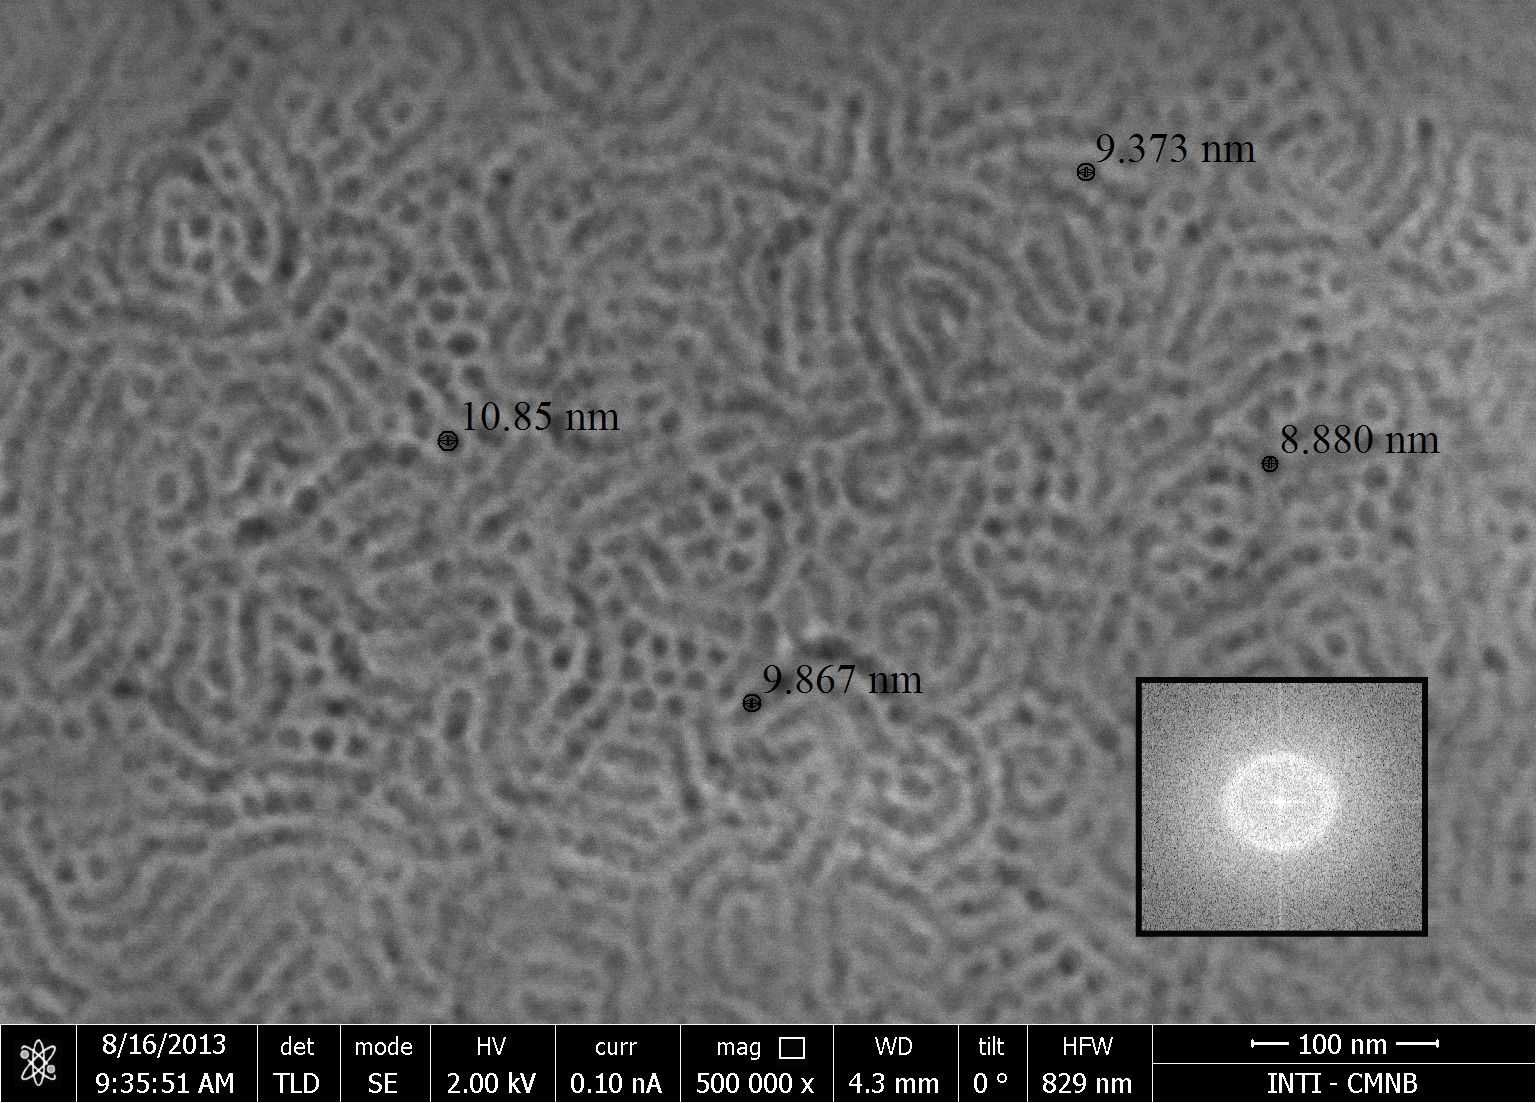
\includegraphics[width=\textwidth]{Imagenes/Superficie-F127-medidas.jpg}
			       		\caption{Microscopía electrónica donde se observa la superficie\index{superficie} de una \pdmF\space con poros de 10nm de diámetro en promedio.}
			       		\label{fig:sem_homogeneidad1}
			       		\end{subfigure}
					\begin{subfigure}[t]{0.49\textwidth}
			 	   	    \includegraphics[width=\textwidth]{Imagenes/Perfil-F127-modificado2.jpg}
			       		\caption{Corte trasnversal porFIB\index{FIB} de una \pdmF\space desde se puede medir el espesor y ver los nanoporos a lo largo del eje trasnversal a la película.}
			       		\label{fig:sem_homogeneidad2}
			       		\end{subfigure}
			       	\begin{subfigure}[t]{0.49\textwidth}
			        	\includegraphics[width=\textwidth]{Imagenes/Superficie-CTAB-medidas.jpg}
			       		\caption{Microscopía electrónica donde se observa la superficie\index{superficie} de una \pdmF\space con poros de 3nm de diámetro en promedio.}
			       		\label{fig:sem_homogeneidad3}
			       		\end{subfigure}
					\begin{subfigure}[t]{0.49\textwidth}
			 	   	    \includegraphics[width=\textwidth]{Imagenes/Perfil-CTAB.jpg}
			       		\caption{Corte trasnversal porFIB\index{FIB} de una \pdmC\space desde se puede medir el espesor de la película. Los nanoporos no se llegan a observar por ser de tamaño muy pequeño para la técnica utilizada.}
			       		\label{fig:sem_homogeneidad4}
			       		\end{subfigure}	
					 \caption[MEB \pdmC\space y \pdmF.]{Microscopia para sistemas de sílice porosos con CTAB y F127 calcinados sobre silicio\index{silicio} con electrodos de Cr\index{cromo}\textbar Au\index{oro} (a y c). Secciones transversales donde se puede apreciar la homogeneidad en el espesor de las películas (b y d).}
					 \label{fig:sem_homogeneidad}	
				     \end{figure}

		El control del espesor se logra variando las condiciones de aceleración y velocidad final del \textit{spin-coater}. Las rampas utilizadas se muestran en la figura \ref{fig:spin}, pág \pageref{fig:spin}, en el gráfico de la figura \ref{fig:esp} se muestra la curva de espesores que corresponde a un sistema nanoporoso de SiO$_2$ utilizando F127 como surfactante\index{surfactante}. 

		Según algunos autores, el tratamiento teórico para el deposito de películas poliméricas por \textit{spin-coating}\index{spin@\textit{spin-coating}} revela una dependencia del espesor con la velocidad según \cite{Norrman2005,Meyerhofer1978,Bornside1989,Lora1990}:
						\begin{equation}
			 			    t = k_1 \omega^{\alpha}
			 		    	 \label{eq:spin_meso}
							\end{equation}
		donde $k_1$ y $\alpha$ son constantes empíricas que dependen que depende de muchos parámetros; de la concentración del monómero, del solvente, del sustrato, de la interacción sol/sustrato y, por supuesto de las propiedades reológicas del sol. Tal como se mostró en la la ecuación \ref{eq:spin}, pág. \pageref{eq:spin} y siguiendo los reportes de la literatura, el valor de $\alpha$ parece mantenerse contante y en las cercanias de $\alpha=0.5$ para una gran cantidad de polímeros. Ajustando los valores del gráfico \ref{fig:esp} se obtienen los valores de $k_1=6413$ y  $\alpha=-0.442$, los cuales siguen la tendencia esperada; disminución del espesor con el aumento de la velocidad angular\index{velocidad!angular} y decaimiento exponencial con $\alpha \approx 0.5$. \marginpar{Quizás acá debe hacer la curva de calibración de espesores para el CTAB, que no la tengo.}
			\begin{figure}[!ht]
						\begin{center}
						\includegraphics[width=0.70\textwidth]{Graficos/Esp_F127.pdf}
						\caption[Espesor en función de la velocidad de rotación\index{velocidad!de rotación}.]{Espesor en función de la velocidad de rotación\index{velocidad!de rotación} para sistemas \pdmF con velocidades angulares comprendidas en 1000 y \SI{4000}{\min^{-1}.}}
						\label{fig:esp}
						\end{center}
						\end{figure}

		La medición de los espesores se realizó parametrizando los datos elipsométricos, para más detalles sobre la técnica consulta la sección \ref{sec:elipso}, pág. \pageref{sec:elipso}.
		%explicar lo del platino\index{platino} en el l capitulo 2, seccionFIB\index{FIB}
		
	\subsection{Discusión sobre la adherencia\index{adherencia} de las \pdm}	

		Se ha demostrado la producción de películas delgadas mesoporososas de sílice (tanto con F127 como con CTAB) en numerosos trabajos sobre sustratos de vidrio\index{vidrio} ó silicio\index{silicio} y nunca se han reportados problemas de adherencia\index{adherencia} \cite{Angelome2008,Fuertes2010,Violi2015}; es más, se conoce que luego de tratamientos térmicos para condensar y calcinar el surfactante\index{surfactante}, las películas sufren una contracción axial\index{contracción axial}a lo largo del eje normal a la superficie\index{superficie} del sustrato\index{sustrato} debido a la fuerte adherencia\index{adherencia} al sustrato.\cite{Soler-Illia2012,Martinez2009}\marginpar{revisar citas} Sin embargo, se sabe desde hace décadas, que los metales nobles no tienen una buena adherencia\index{adherencia} sobre sustratos no-metálicos\cite{Kern1990,Hieber1976}, con lo cual es de esperar que también se experimenten problemas de adherencia\index{adherencia} al querer depositar un sol\index{sol} sobre una película delgada \index{película!delgada}de Au. 

		\subsubsection{Adherencia en electrodos de Au\index{electrodo!de Au}}

			En el caso del Pluronic F127\index{Pluronic F127} sobre películas de Au, se observó, en algunos casos, falta de adherencia. En el gráfico \ref{fig:adherencia_F127} vemos un ejemplo en el cual se <<despega>> la película durante la impregnación de la película con \aminorutenio. La forma del voltagrama (tanto los cambios en la intensidad como los corrimientos en el potencial) se discuten en profundidad en el capitulo \ref{chap:Electroquimica}, por ahora nos basta con decir que se trata de un cambio repentino de un ciclo al siguiente, pasando de la típica respuesta de una película mesoporosa\index{película!mesoporosa} a la respuesta habitual de un electrodo desnudo de Au, indicador de que la película no sufrió un disolución lenta y paulatina, sino que se desprendió del sustrato, total o parcialmente, en algún momento de la medición.
				\begin{figure}[th]
				 	   	    \begin{center} 
				        	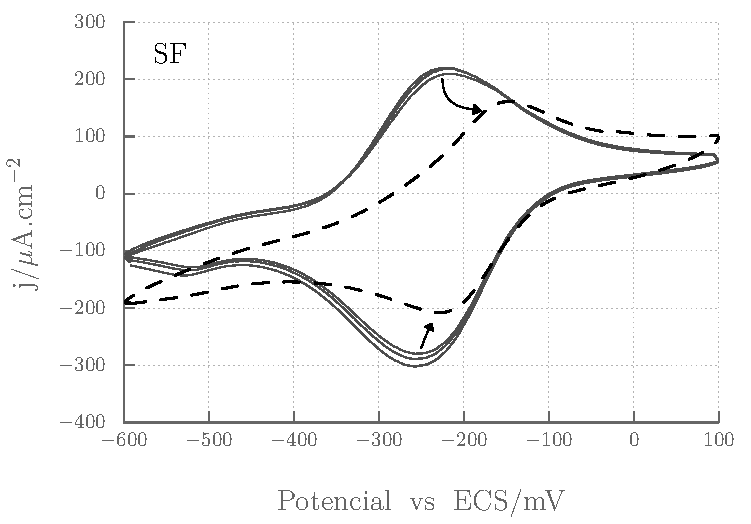
\includegraphics[width=0.70\textwidth]{Graficos/Adherencia_F127.pdf}
				       		\caption[Adherencia de \pdmF \space sobre una película delgada \index{película!delgada}de Au.]{Voltamperometría cíclica, compuesta por ciclos consecutivos donde se evidencia la falta de adherencia\index{adherencia} de \pdmF \space sobre electrodo de Au\index{electrodo!de Au}. Las VC fueron tomadas a \SI{50}{\milli\volt.\second^{-1}} usando de referencia ESC.}
				         	\label{fig:adherencia_F127}
				     		\end{center}
				     		\end{figure}

			En el caso del CTAB el comportamiento es algo diferente. Se ven problemas de adherencia\index{adherencia} en la mayoría de los tratamientos alternativos, así como en la calcinación\index{calcinación}, tanto de grietas y fisuras como de desprendimiento antes de someter los sensores\index{sensor} a cualquier medición, es decir, apenas terminada la síntesis. Solo se rescataron algunos casos exitosos de formación de \pdmC\space utlizando como soporte electrodos de Au\index{electrodo!de Au}. Estos sirvieron para hacer experimentos de EQ conceptuales sobre transporte\index{transporte} en poros (consultar capitulo \ref{chap:Electroquimica}), pero en la generalidad de los casos se observa desprendimiento de la película tal como muestran las imágenes de la figura \ref{fig:CTAB_adherencia}.
	     
				\begin{figure}[th]
		 	   	    \begin{subfigure}[t]{0.49\textwidth}
			        	\includegraphics[width=\textwidth]{Imagenes/Au_FCCTAB_adherencia1.jpg}
			       		\end{subfigure}
					\begin{subfigure}[t]{0.49\textwidth}
			 	   	    \includegraphics[width=\textwidth]{Imagenes/Au_FCCTAB_adherencia2.jpg}
			       		\end{subfigure}
					 \caption[Adherencia de CTAB sobre electrodos.]{Microscopías electrónicas donde se muestra la falta de adherencia\index{adherencia} de \pdmC \space sobre una película delgada \index{película!delgada}de Au.}
					 \label{fig:CTAB_adherencia}	
				     \end{figure}
			Además de la ya mencionada falta de adherencia\index{adherencia} de los no-metales sobre películas de Au, este desprendimiento se debe, sobre todo, a la interacción CTAB-Au. Es numerosa la información que se encuentra en la literatura sobre la interacción superficial de CTAB sobre superficie\index{superficie}s de nanoparticula\index{nanoparticula}s y películas delgadas de Au\cite{Cheng2003,Smith2008,Lim2014,Meena2013,Wang2013,Hamon2009}. Su uso extendido se basa en la adsorción\index{adsorción} y autoensamblado del CTAB para controlar el crecimiento y estabilización de nanoparticula\index{nanoparticula}s de Au. Más allá de la concentración miscelar crítica (cmc) se adsorben las miscelas sobre la superficie\index{superficie}, su distribución y densidad parece depender de factores como la concentración, la orientación cristalina del Au, el solvente, tamaño de las nanoparticula\index{nanoparticula}s y rugosidad\index{rugosidad} de la superficie\index{superficie}\cite{Meena2013,Lim2014}. La adsorción\index{adsorción} de estas miscelas en la superficie\index{superficie}, sumada a la poca adherencia\index{adherencia} del SiO$_2$, es lo que impide la formación y adherencia\index{adherencia} de \pdmC\space sobre electrodos de Au\index{electrodo!de Au}.
		
			%Agregar mas adelante que se puede utilizar para sistemas mas adelante como bicapa sobre F127, demostrado en otros paper bla bla y poner bibliografía. Anduvo en parte para el calcinado.
							
		\subsubsection{Modificaciones superficiales}\label{sec:adherencia}

			La adherencia\index{adherencia} de las \pdm\space es crítica para la elaboración de los sensores, y, en función de los resultados expuestos en la sección anterior, es un problema a tener en cuenta durante la fabricación de sensores\index{sensor} electroquímico\index{electroquimico}s\index{electroquimico} basados en electrodos de Au\index{electrodo!de Au}.

			Las estrategias usadas para solucionar estos problemas se basaron en dos conceptos:
				\begin{enumerate}

					\item En la modificación superficial de los electrodos generando puntos de anclaje al esqueleto inorgánico.

					\item Minimizando el área de contacto electrodo-mesoporoso.

					\end{enumerate}
			La modificación superficial de los electrodos se llevó acabo siguiendo el procedimiento detallado en el capitulo \ref{chap:Materiales}, sección \ref{sec:silanizacion}. Se buscó una molécula compatible con el sistema utilizado, que pueda vincular la superficie\index{superficie} del electrodo e integrarse en el esqueleto de las \pdm. Se usó para este fin el 3-mercaptopropil trimetoxisilano\index{mercaptopropil@3-mercaptopropil trimetoxisilano} (MPTMS), el cual es fácilmente de ligar covalentemente al Au\cite{Gosser} por el tiol, y por el otro tiene el silano el cual es perfectamente compatible con el precursor\index{precursor} utilizado\cite{Wu2014,Wu2013,Chen2011}. En la figura \ref{fig:mod_sup} se muestra la molécula de MPTMS y un esquema de como queda anclado la \pdm\space al electrodo.
					\begin{figure}[!ht]
							\begin{center}
							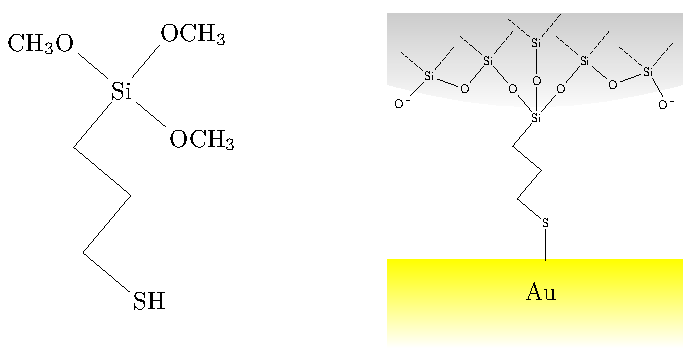
\includegraphics[width=0.70\textwidth]{Esquemas/mod_sup.pdf}
							\caption[Modificación superficial de los electrodos.]{Izquierda: Molécula de  3-mercaptopropil trimetoxisilano\index{mercaptopropil@3-mercaptopropil trimetoxisilano} utilizada como ligante entre los electrodos y las \pdm. Derecha: Esquema pictórico de la modificación superficial con MPTMS.}
							\label{fig:mod_sup}
							\end{center}
							\end{figure}
			Una vez realizada la modificación superficial se hicieron comparaciones con electrodos sin modificar, para evaluar el posible bloqueo de los electrodos. La figura \ref{fig:comparaciones_MPTMS} se muestran los voltagramas donde se comparan las superficie\index{superficie}s modificadas con MPTMS y sin MPTMS, recubiertas con \pdm\space y sin recubrir. De estos gráficos comparativos se desprende que el rendimiento electroquímico\index{electroquimico} no se ve afectado significativamente.
	 			\begin{figure}[th]
		 	   	    \begin{subfigure}[t]{0.49\textwidth}
			        	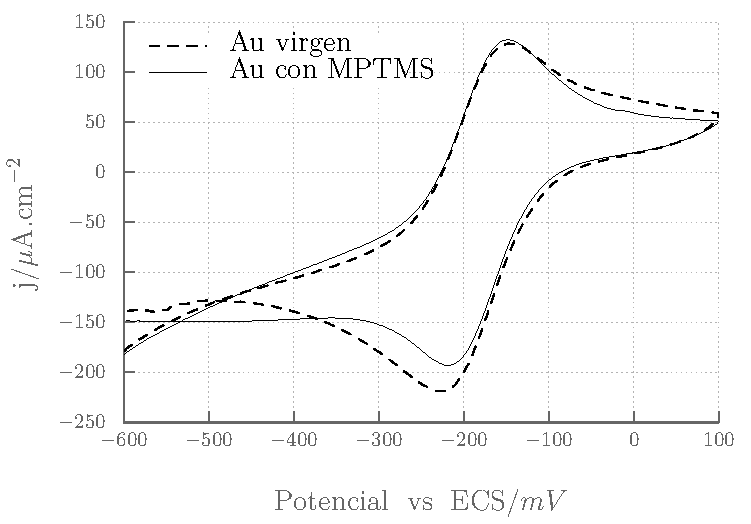
\includegraphics[width=\textwidth]{Graficos/Comparacion_Au-MPTMS.pdf}
			       		\caption{Electrodo desnudo de Au\index{oro} comparado con uno modificado con MPTMS.}		 
			       		\end{subfigure}
					\begin{subfigure}[t]{0.49\textwidth}
			 	   	    \includegraphics[width=\textwidth]{Graficos/Comparacion_F127-MPTMS.pdf}
			       		\caption{\pdmF\space sobre electrodo de Au\index{electrodo!de Au}\index{oro} tratados con MPTMS y sin tratar.}
			       		\end{subfigure}
					 	\caption[Comparacion de superficie\index{superficie}s con y sin MPTMS.]{Voltametrias cíclicas para \aminorutenio\space \SI{1}{\milli\Molar} realizados a \SI{50}{\milli\volt.\second^{-1}} comparando los resultados de electrodos modificados con MPTMS y sin modificar.}
					 \label{fig:comparaciones_MPTMS}	
				     \end{figure}
			La segunda opción que se tuvo en cuenta, para promover una mayor adherencia\index{adherencia} de las \pdm\space a los sensores, se basa en minimizar el área de contacto electrodo-mesoporoso. Las resultados de los experimentos discutidos en este capitulo fueron derivados de \pdm\space sobre electrodos plenos de Au. Sin embargo, los sensores\index{sensor} son un conjunto de electrodos o microelectrodo\index{electrodo!microelectrodo}s sobre un sustrato\index{sustrato} no-metalico (p. ej. SiO$_2$ o vidrio). Eligiendo un diseño adecuado se puede minimizar el área de los electrodos respecto del soporte, de esta forma las \pdm\space quedan adheridas fuertemente a los sectores donde no está el Au. El resultado final es una película bien adherida sobre una superficie\index{superficie} mixta soporte/electrodos.  La figura \ref{fig:adherencia_microelectrodo} representa esta situación.
				\begin{figure}[!ht]
					\begin{center}
					\includegraphics[width=0.70\textwidth]{Esquemas/adherencia_microelectrodo.pdf}
					\caption[Adherencia a los microelectrodo\index{electrodo!microelectrodo}s.]{Corte transversal de los sensores\index{sensor} donde se observan los microelectrodo\index{electrodo!microelectrodo}s y la \pdm depositada, allí se indican las zonas de baja y alta adherencia.}
					\label{fig:adherencia_microelectrodo}
					\end{center}
					\end{figure}
			Ambas estrategias que promueven la adherencia\index{adherencia} de las \pdm\space son complementarias. Esto quiere decir que se puede optimizar un diseño para minimizar los electrodos y, a su vez, se pueden tratar con MPTMS como puntos de vinculación entre el mesoporosos y el electrodo. En este caso el tratamiento se realiza luego de depositar el Au\index{oro} y antes de realizar el decapado de la fotorresina (consultar sección \ref{sec:fotolito}, pág. \pageref{sec:fotolito}).		
			% Por último decir que se van a usar de ahora en adelante estos sistema, reforzar con bibliografia.

	\subsection{Análisis de la porosidad}

		Dentro del los objetivos de esta primera etapa se incluyó el de evaluar las propiedades de porosidad\index{porosidad} de las películas; ya que, como veremos mas adelante a la largo de la tesis, la porosidad\index{porosidad} y accesibilidad\index{accesibilidad} son los parámetros que nos determinarán la cantidad de analito que se adsorbe en la misma. 

		Del estudio de las películas porSEM\index{SEM} se puede obtener información muy valiosa como tamaño y distribución de los poros\index{distribución!de poro}, así como estudios de la organización cristalina de los mismos.\marginpar{faltan citas.} En nuestro caso se obtienen, coincidiendo la con información existente en la literatura, arreglos con orden local para el \pdmF. Como se muestra en en los ejemplos de la figura \ref{fig:F127_Si_Au}.

			\begin{figure}[th]
		 	   	    \begin{subfigure}[t]{0.49\textwidth}
			        	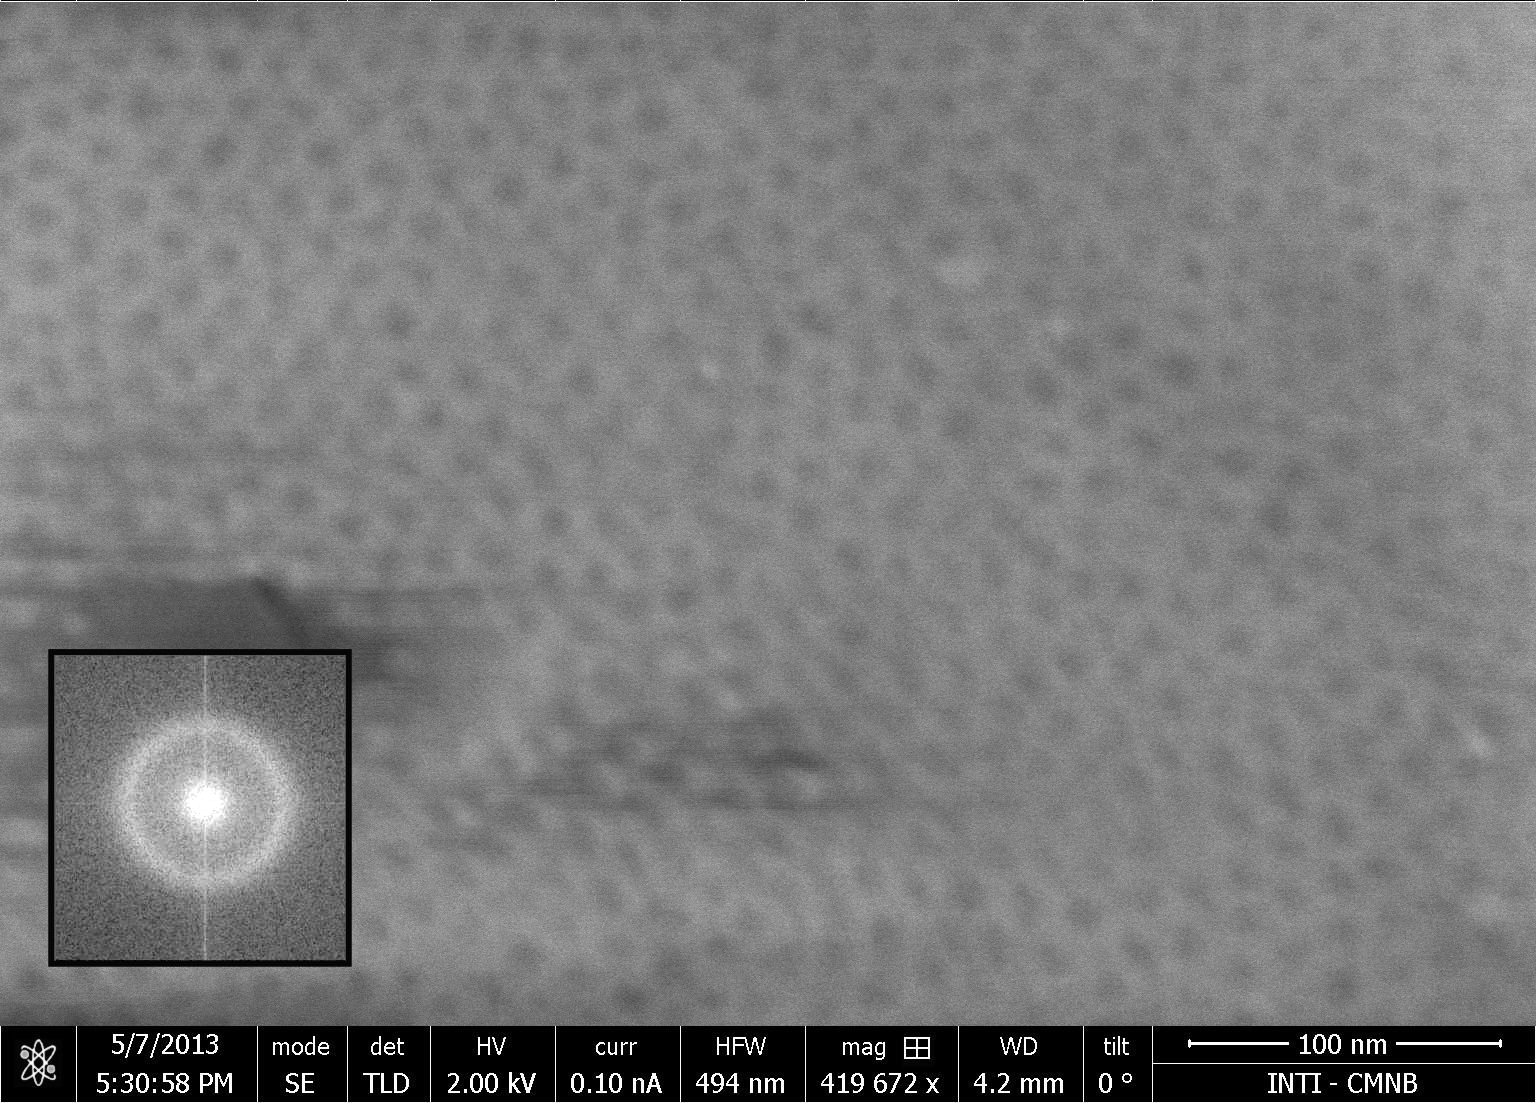
\includegraphics[width=\textwidth]{Imagenes/F127_Si_sup.jpg}
			       		\end{subfigure}
					\begin{subfigure}[t]{0.49\textwidth}
			 	   	    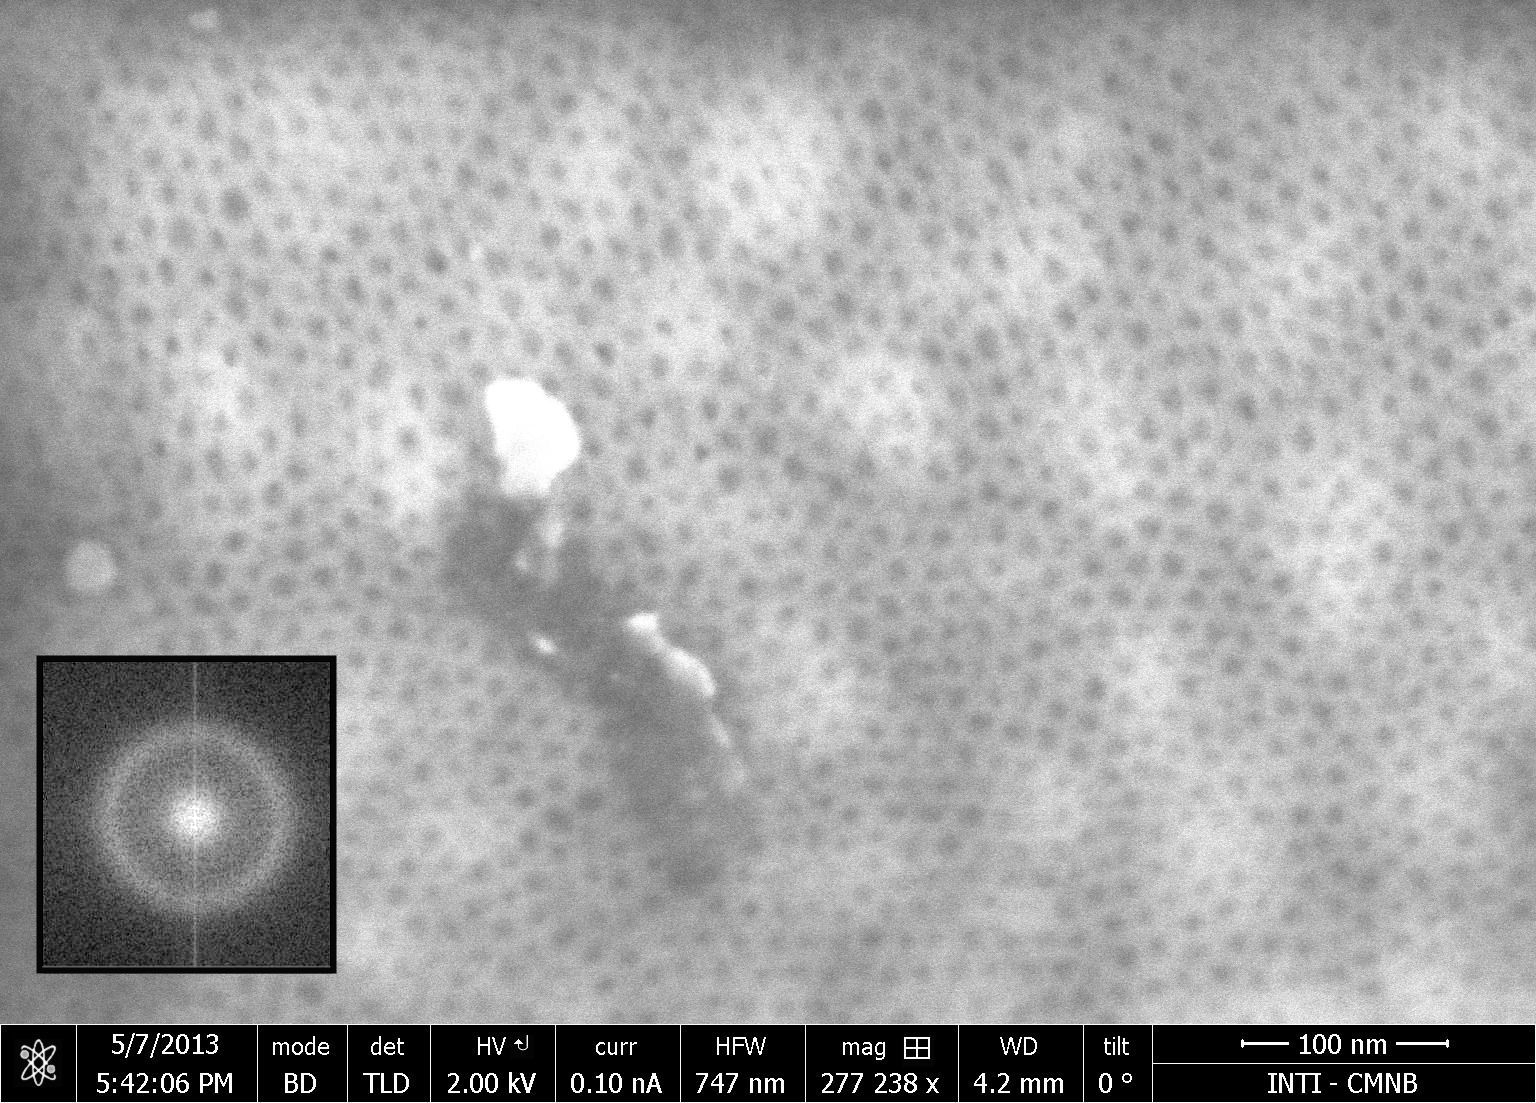
\includegraphics[width=\textwidth]{Imagenes/F127_Au_sup.jpg}
			       		\end{subfigure}
					\caption[SEM arreglo poroso sobre Si y Au.]{Microscopía electrónica de barrido de una \pdmF\space donde se observa la distribución y homogeneidad de los poros en superficie\index{superficie}. Izquierda: sobre sustrato\index{sustrato} de silicio. Derecha: sobre sustrato\index{sustrato} de Au.}	 
					 \label{fig:F127_Si_Au}
					 \end{figure}

		En el caso de las películas estructuras con CTAB es más difícil hacer una análisis porSEM\index{SEM}, ya que el diámetro de los poros ($\approx$ \SI{3}{\nm}) esta sobre el limite de la técnica y solo se puede ver que existe un sistema de poros (ver figura \ref{fig:sem_homogeneidad3}). En este caso, para hacer un estudio por imágenes mas completo, se debería recurrir a microscopia\index{microscopía} electrónica de transmisión\index{microscopía!de transmisión}.

		El estudio porSEM\index{SEM} es sumamente útil en muchos aspectos; sin embargo la información que nos brinda es de áreas muy pequeñas, superficial y no nos dice nada sobre la conectividad\index{conectividad} y cuello\index{cuello de poro}s de las películas.  Es por ello recurrió a la técnica de elipsoporosimetría ambiental (PEA), la cual es una técnica promedio donde podemos obtener información valiosa sobre la accesibilidad\index{accesibilidad} del agua a los poros, volumen poroso de las \pdm, distribución de tamaños de poros y cuello\index{cuello de poro}s y variación del espesor en función de la presión de vapor\index{presión de vapor} de agua relativa a la presión de saturación (P/Ps). Los detalles experimentales de esta técnica se presentaron en el capitulo \ref{sec:elipso}, pág. \pageref{sec:elipso}. Los cálculos realizados para obtener información estructural a partir de las isoterma\index{isoterma}s se basaron en el protocolo detallado en dos trabajos del grupo de ClémentSánchez\index{Sánchez} \cite{Boissiere2005,Sakatani2006}.

		En las figuras \ref{fig:F127_EPA} y \ref{fig:CTAB_EPA} se presentan las isoterma\index{isoterma}s de adsorción\index{adsorción} de agua para sistemas calcinados \pdmF\space y \pdmC. Se observa que ambas son de tipo IV, según la clasificación de Brunauer\index{Brunauer}\cite{Gregg1967,Violi2015,Fuertes2010}. Este tipo de isoterma\index{isoterma}s con histéresis entre la rama de adsorción\index{adsorción} y la de desorción\index{desorción} es característica de materiales con mesoporos, donde los poros se llenan por condensación\index{condensación} capilar. Por otro lado el ciclo de histéresis es de tipo H1, según la clasificación IUPAC\cite{Gregg1967,Lowell2004,Sing1985a}, lo cual indica poros de tamaño uniforme.

		     	  	\begin{figure}[!ht]
		     	  		\begin{subfigure}[t]{0.495\textwidth}
		     	  		\includegraphics[width=\textwidth]{Graficos/SI_F127_Calcinado_EPA.pdf}
						\caption[Elipsoporsimetría \pdmF\space calcianda.]{Elipsoporsimetría de una \pdmF\space sobre sustrato\index{sustrato} de silicio\index{silicio} sintetizada por el método clásico de calcinación\index{calcinación}.}
						\label{fig:F127_EPA}
						\end{subfigure}
						\begin{subfigure}[t]{0.495\textwidth}
		     	  		\includegraphics[width=\textwidth]{Graficos/SI_F127_Calcinado_PSD.pdf}
						\caption[Distribución \pdmF.]{Distribución de tamaño de poro\index{poro} y cuello\index{cuello de poro} para una \pdmF\space.}
						\label{fig:F127_PSD}
						\end{subfigure}
						\caption[Elipsoporosimetría para sistemas \pdmF.]{Distribución de poros y cuello\index{cuello de poro}s (b) y curva de adsorción\index{adsorción}/desorción de agua para una \pdmF (a), la misma corresponde a una isoterma\index{isoterma} de tipo IV con un lazo de histéresis de tipo H1, lo cual se concuerda con materiales mesoporosos con tamaño de poros uniformes, de aproximadamente \SI{10}{\nm}.}
						\end{figure}
					\begin{figure}[!ht]
		     	  		\begin{subfigure}[t]{0.495\textwidth}
		     	  		\includegraphics[width=\textwidth]{Graficos/SI_CTAB_Calcinado_EPA.pdf}
						\caption[Elipsoporsimetría \pdmF\space calcianda.]{Elipsoporsimetría de una \pdmF\space sobre sustrato\index{sustrato} de silicio\index{silicio} sintetizada por el método clásico de calcinación\index{calcinación}.}
						\label{fig:CTAB_EPA}
						\end{subfigure}
						\begin{subfigure}[t]{0.495\textwidth}
		     	  		\includegraphics[width=\textwidth]{Graficos/SI_CTAB_Calcinado_PSD.pdf}
						\caption[Distribución \pdmC.]{Distribución de tamaño de poro\index{poro} y cuello\index{cuello de poro} para una \pdmC\space.}
						\label{fig:CTAB_PSD}
						\end{subfigure}
						\caption[Elipsoporosimetría para sistemas \pdmC.]{Distribución de poros y cuello\index{cuello de poro}s (b) y curva de adsorción\index{adsorción}/desorción de agua para una \pdmC (a), la misma corresponde a una isoterma\index{isoterma} de tipo IV con un lazo de histéresis de tipo H1, lo cual se concuerda con materiales mesoporosos con tamaño de poros uniformes, de aproximadamente \SI{3}{\nm}.}
						\end{figure}	
		
		A medida que la presión de vapor\index{presión de vapor} externa aumenta, la adsorción\index{adsorción} en los mesoporos se produce a través de la formación de una monocapa y luego de multicapas de moléculas de agua sobre las paredes de los poros, seguida de condensación\index{condensación} capilar, es decir, llenado de los poros con agua líquida. La posterior disminución de la presión externa resulta en la desorción\index{desorción} mediante evaporación capilar, vaciando el centro de los poros, seguida por la desorción\index{desorción} de la multicapa	de solvente de las paredes de los poros. La expresión cuantitativa de la condensación\index{condensación} capilar esla ecuación de Kelvin\index{Kelvin}, (ecuación \ref{eq:kelvin}), que es la base de los procedimientos de cálculo de distribución de tamaño de poro\index{poro} a partir de isoterma\index{isoterma}s de tipo IV.\cite{Baklanov2000}
		
		En las figuras \ref{fig:F127_EPA} y \ref{fig:CTAB_EPA} se graficaron los indices de refracción ($n$) y la fracción porosa ocupada por agua adsorbida (V$_{ads}$/V$_p$) en función de la presión de vapor\index{presión de vapor} de aguar relativa a la presión de saturación (P/P$_s$). 

		En las figuras \ref{fig:F127_PSD} y \ref{fig:CTAB_PSD} se muestran se muestran las distribuciones de tamaño de poro\index{poro} para estos sistemas. Estas distribuciones se obtuvieron a partir de las isoterma\index{isoterma}s, y se extrajo información estructural tanto de la rama de adsorción\index{adsorción} como de la de desorción\index{desorción}.

	\subsection{Análisis por FTIR}\label{sec:Analisis_IR}

		Son muchos los trabajos en los cuales se estudia la respuesta de películas delgadas de SiO$_2$ en IR\cite{Olsen1989,Almeida1990,Redol1997,Innocenzi2003}, y también muchos que otros que hacen usos de estos resultados \cite{Angelome2008,Calvo2008,Calvo20210}.
		El análisis de espectroscopia\index{espectroscopia} infrarroja por transformada de Fourier (FTIR) se utilizó en esta tesis para identificar y caracterizar la estructura inorgánica porosa de SiO$_2$, evaluar comparativamente condensación\index{condensación} del óxido, y determinar la presencia de residuos de surfactante\index{surfactante}. Como veremos en el siguiente capítulo, las películas no serán sometidas a calcinación\index{calcinación}, sino que se remueve el surfactante\index{surfactante} por extracción\index{extracción}, por ello es de mucha ayuda el seguimiento por FTIR\index{FTIR} de la presencia de surfactante\index{surfactante}. 

			\begin{figure}[!ht]
						\begin{center}
						\includegraphics[width=\textwidth]{Graficos/IR_Denso.pdf}
						\caption[FTIR SiO$_2$ denso y SiO$_2$ mesoporoso.]{Espectro de absorción de IR de una película SiO$_2$ denso comparada con una de SiO$_2$ mesoporoso. Se observa la aparición de un marcado hombro a mayores frecuencias sobre el pico del modo LO$_3$, y la aparición de un pico correspondiente a la vibración\index{vibración} Si-OH.}
						\label{fig:IR-denso}
						\end{center}
						\end{figure}

		PlinioInnocenzi\index{Innocenzi}\cite{Innocenzi2003} hace un análisis completo y bien fundamentado sobre las vibraciones\index{vibración} en el IR, con incidencia normal y haz trasmitido, de películas delgadas de SiO$_2$ tanto densas como porososas. Analiza, para los enlaces Si-O-Si, la presencia de 4 modos de vibración\index{vibración} óptico-trasversales (TO$_x$) y 4 modos óptico-longitudinales (LO$_x$) para películas delgadas de SiO$_2$. Al\index{aluminio} ser la incidencia del haz, normal a la superficie\index{superficie}, solo deberían exitarse las vibraciones\index{vibración} óptico-transversales, sin embargo se observan banda de vibraciones\index{vibración} correspondientes a modos optico-longitudinales asociadas a oscilaciones colectivas acopladas TO-LO.\cite{Pai1986,Grosse1986,Innocenzi2003}.

		El modo TO$_1$, presenta una banda débil $\approx$\SI{460}{\cm^{-1}} asociada a movimientos de balanceo; el modo TO$_2$ está asociado a un estiramiento simétrico con un pico débil cercano a $\approx$\SI{800}{\cm^{-1}}; y el modo TO$_3$, el cual presenta un pico intenso centrado en $\approx$\SI{1075}{\cm^{-1}}, se encuentra asociado a las vibraciones\index{vibración} asimétricas del enlace Si-O-Si. Respecto de los modos ópticos-longitudinales, LO$_1$ y LO$_2$ no son visibles, y LO$_3$, aparece como un hombro de la banda TO$_3$ a mayores frecuencias. La observación experimental de los modos TO$_4$ y LO$_4$ es escasa, cuando se observa aparecen como bandas débiles en la zona comprendida entre 1200 y \SI{1150}{\cm^{-1}} \cite{Pai1986,Grosse1986}.
		
				\begin{figure}[!ht]
						\begin{center}
						\includegraphics[width=\textwidth]{Graficos/IR_F127.pdf}
						\caption[FTIR para una \pdmF.]{Espectro de absorción para una \pdmF\space antes y después de calcinar, donde se puede apreciar la aparición de un pico fuerte el cual correspondiente al surfactante\index{surfactante} F127.}
						\label{fig:IR_F127_calciando}
						\end{center}
						\end{figure}
				
				\begin{figure}[!ht]
						\begin{center}
						\includegraphics[width=\textwidth]{Graficos/IR_CTAB.pdf}
						\caption[FTIR para una \pdmC.]{Espectro de absorción para una \pdmC\space antes y después de calcinar, donde se puede apreciar la aparición de un pico fuerte el cual correspondiente al surfactante\index{surfactante} CTAB.}
						\label{fig:IR_CTAB_calcinado}
						\end{center}
						\end{figure}

		Otra de las observaciones relevante, realizadas por Al\index{aluminio}meida y Pantano\cite{Almeida1990}, es el hecho que de que la naturaleza del hombro presente en $\approx$\SI{1180}{\cm^{-1}}	corresponde a una mezcla de los modos LO$_3$ y TO$_3$, con predominancia de carácter LO, y se intensifica con el aumento de la porosidad\index{porosidad} de la película. Este fenómeno parece estar asociado a la dispersión de la radiación\index{radiación} IR dentro de los poros y la consecuente activación del modo longitudinal.

		Esta observación se puede corroborar en la figura \ref{fig:IR-denso}, donde se compara una \pdm\space con una película delgada \index{película!delgada}de SiO$_2$ depositada por \textit{sputtering}\index{sputtering@\textit{sputtering}}.  Al\index{aluminio}lí se ve el hombro bien acentuado para la \pdm\space y una banda en en $\approx$\SI{965}{\cm^{-1}} asociada al estiramiento Si-OH/Si-O$^-$; mientras que para la película de SiO$_2$ denso se observa que aparece la incipiente banda de LO$_4$ y desaparece la banda del Si-OH/Si-O$^-$
				
		Por otro, cuando se analiza la presencia del surfactante\index{surfactante}, se centrará la atención en las bandas que corresponden a las vibraciones\index{vibración} del enlace C-H, las cuales aparecen en la zona de $\approx$\SI{965}{\cm^{-1}}. En la figuras \ref{fig:IR_F127_calciando} y \ref{fig:IR_CTAB_calcinado} se comparan \pdm\space calcinadas y sin calcinar para los surfactante\index{surfactante}s utilizados. Se ve como desaparecen las bandas correspondientes a al vibración\index{vibración} C-H debido a la calcinación\index{calcinación} del surfactate; se conserva la forma del hombro a $\approx$\SI{1180}{\cm^{-1}} coincidente con una estructura porosa y se observa la banda en en $\approx$\SI{965}{\cm^{-1}} asociada al estiramiento Si-OH/Si-O$^-$, el cual según algunos autores desaparece sólo cuando las películas se someten a T$>$\SI{500}{\celsius}.\cite{Innocenzi2003,Almeida1990,Bertoluzza1982}
	
		Toda las medidas fueron llevadas a cabo con el microscopio asociado al equipo de FTIR\index{FTIR} y en modo reflexión, los detalles experimentales fueron explicados en la sección \ref{sec:IR}, \pageref{sec:IR}. %En la tabla que sigue se hace un resumen de las bandas observadas y su correpondiente asignación.
		\marginpar{tabla con las vibraciones\index{vibración} y los modos???}

			%Tabla???
			%Comparacion relacion picos si-o-si / si-oh 

	\subsection{Accesibilidad de las PDM}

			Hasta ahora se han evaluado muchos de los aspectos fundamentales para poder pensar en las películas mesoporosas de óxido de silicio\index{silicio!oxido de}, como sensores; la accesibilidad\index{accesibilidad} de los poros, el volumen poroso, los sustratos, la técnica de deposito, control del espesor, etc. 

			Sin embargo, se debe tener en cuenta un aspecto crítico para utilizar estas películas como parte de un sensor\index{sensor} electroquímico\index{electroquimico}, y, este es, el libre acceso de los analitos a través de los nanoporos, de forma de poder difundir hasta la superficie\index{superficie} del electrodo, y, que tenga lugar allí, la reacción electroquímica\index{electroquimico}.

			Para ello, basta con colocar una solución, con una sonda\index{sonda} electroquímica\index{electroquimico} adecuada, en la celda de medición. La forma en que fueron tomadas las medidas se explica en la sección \ref{sec:medidas_eq}, pág \ref{sec:medidas_eq}. La figura \ref{fig:accesibilidad} muestra una señal electroquímica\index{electroquimico} intensa, para \aminorutenio\space \SI{0.315}{\milli\Molar} en solución de KCl \SI{0.1}{\Molar}, lo que indica que la superficie\index{superficie} del electrodo se encuentra accesible. Los resultados sugieren que existe un camino percolativo en la \pdm, tanto si se estructuran con F127 o con CTAB, que permite, o bien que la señal electroquímica\index{electroquimico} se propague desde el seno de la solución hasta el electrodo o bien que el analito difunda desde la solución al electrodos.   Los fenómenos de trasporte involucrados en este experimento, son tema central de esta tesis y se discuten en detalle en el capitulo \ref{chap:Electroquimica}, asi como la forma de los voltagrama, allí se analiza la separación del potencial entre los picos anódico y catódico y las intensidades de los mismos relativa a un electrodo de Au\index{electrodo!de Au}\index{oro} sin recubrir. \marginpar{Falta un experimento que pueda demostrar accesibilidad\index{accesibilidad} para películas CTAB.}

						\begin{figure}[th]
				 	   	    \begin{center} 
				        	\includegraphics[width=0.70\textwidth]{Graficos/Accesibilidad-electrodo.pdf}
				       		\caption[Accesibilidad electrodo de trabajo\index{electrodo!de trabajo}.]{Voltametría Cíclica de \aminorutenio\space \SI{0.315}{\milli\Molar} sobre un electrodo de Au\index{electrodo!de Au}\index{oro} recubierto \pdmF\space con una velocidad de barrido\index{velocidad!de barrido} \SI{50}{\milli\volt.\second^{-1}} usando de referencia ESC.}s
				         	\label{fig:accesibilidad}
				     		\end{center}
				     		\end{figure}

			%El fenomeno de transporte\index{transporte} de sonda\index{sonda}s electroquimicas a través de las \pdm\space es un tema cemtral de este trabajo y se trata en profundidad en el capitulo.... por ahora 
			%Por tecnicas de VC. Distinguir entre accesibilidad\index{accesibilidad} de los poros y accesibilidad\index{accesibilidad} para llegar al electrodo y un camino de percolación para llegar al fondo.

\section{Conclusiones parciales}

En este capitulo se presentan los primeros resultados que se obtuvieron en el proceso de fabricación, desarrollo y caracterización de los sensores\index{sensor} electroquímico\index{electroquimico}s\index{electroquimico} permeoselectivos basados en películas delgadas de óxido de silicio\index{silicio!oxido de}. Se lograron sintetizar las películas mesoporosas de óxido de silicio\index{silicio!oxido de}\index{silicio} sobre diferentes sustratos, silicio, vidrio, oro\index{oro} y microelectrodo\index{electrodo!microelectrodo}s. Se utilizaron dos agentes moldeantes F127 y CTAB y seguió la vía clásica de calcinación\index{calcinación} a \SI{350}{\celsius} para condensación\index{condensación} del SiO$_2$ y calcinación\index{calcinación} del surfactante\index{surfactante}. Teniendo en cuenta las herramientas y procesos propios de la microelectronica, para el deposito del sol, se eligió usar exclusivamente el método de \textit{spin-coating}\index{spin@\textit{spin-coating}}. Se regulo el espesor de las películas al deseado, entre 200 y \SI{250}{\nm} para que no se produzcan fracturas y discotinuidades en las películas. Frente a los problemas encontrados de adherencia\index{adherencia} a los electrodos de Au\index{electrodo!de Au} se utilizaron dos estrategias: modificación química y optimización del diseño de los electrodos. Mejorada la adherencia\index{adherencia} se demostró que el desempeño electroquímico\index{electroquimico} no se vio afectado. 

Las películas fueron caracterizadas por microscopia\index{microscopía} electrónica\index{microscopía!electrónica}, elipsoporossimetría, espectroscopia\index{espectroscopia} IR y electroquimicamente. De estas caracterización se demostró que las películas son homogéneas en espesor, en superficie\index{superficie}, de poroso uniformes en tamaño y distribución y que existe un camino percolativo del seno de la solución a la superficie\index{superficie} del electrodo, permitiendo realizar reacciones de óxido/reducción sobre la superficie\index{superficie} del electrodo.


%destacados:

%Control de espesor
%Tecnicas compatible spin-coating
%Sobre Au\index{oro} - todo bien! sobre si / vidrio
% sistemas porosos, accesibles, homogeneos con llegada al electrodo.
% Problemas de adhesion y soolucion con molecula de MPTMS
% Limitaciones!!! Calcinacion....


